\documentclass[conference]{IEEEtran}

% Pacotes para suporte ao Português e imagens
\usepackage[utf8]{inputenc}
\usepackage[T1]{fontenc}
\usepackage[brazilian]{babel}
\usepackage{amsmath,amssymb,amsfonts}
\usepackage{algorithmic}
\usepackage{graphicx}
\usepackage{textcomp}
\usepackage{xcolor}

\begin{document}

\title{Relatório de Práticas em Sistemas Digitais - Laboratório 04}

\author{\IEEEauthorblockN{Lucca, João Vital, Danyel}
\IEEEauthorblockA{\textit{Departamento de Computação (DCOMP)} \\
\textit{Universidade Federal de Sergipe (UFS)}\\
São Cristóvão, Brasil \\
} % Substitua pelo seu email real
}

\maketitle

\begin{abstract}
Este relatório descreve as atividades práticas realizadas no Laboratório 04, que tem como foco a introdução ao simulador SPICE para descrição e análise de circuitos elétricos. Utilizando o software SpiceOpus e uma tecnologia de 0.5$\mu$m, o experimento avalia o comportamento de um inversor CMOS sob diferentes condições paramétricas. O estudo detalha a influência da capacitância de carga e das dimensões do canal (W e L) dos transistores nos tempos de atraso, transição e na dissipação de potência dinâmica do circuito.
\end{abstract}

\begin{IEEEkeywords}
CMOS, SPICE, portas lógicas, análise temporal, capacitância.
\end{IEEEkeywords}

\section{Introdução Teórica}
O desenvolvimento de sistemas digitais modernos exige a validação do comportamento elétrico dos circuitos muito antes de sua fabricação física. A ferramenta SPICE atua exatamente nesse nível mais baixo de abstração, permitindo simular componentes como capacitores, resistores e transistores com alta precisão. 

Neste laboratório, o objeto de estudo é a porta lógica fundamental: o inversor CMOS, composto por um par de transistores PMOS e NMOS. Em um ambiente de simulação, o desempenho desse inversor é avaliado através de suas características temporais:
\begin{itemize}
    \item \textbf{Tempos de transição:} Representados pelo tempo de subida ($T_{rise}$) e tempo de descida ($T_{fall}$) do sinal.
    \item \textbf{Tempos de propagação:} O atraso que o sinal sofre ao cruzar a porta lógica, medido como $T_{plh}$ (propagação de baixo para alto), $T_{phl}$ (propagação de alto para baixo) e o atraso médio de propagação $T_{p}$.
\end{itemize}

Compreender como as dimensões físicas do MOSFET (largura $W$ e comprimento $L$) e a capacitância afetam essas métricas é essencial para o design eficiente de hardware.

\section{Materiais Utilizados}
Para a realização deste laboratório e das simulações, foram empregados os seguintes recursos:
\begin{itemize}
    \item Software simulador SpiceOpus.
    \item Arquivo de modelo de tecnologia de 0.5$\mu$m (\texttt{cmos7tm.mod}).
\end{itemize}

\section{Descrição das Atividades e Resultados}

\subsection{Atividade 01 - Inversor CMOS Padrão}
A prática foi iniciada com a transcrição do netlist (código SPICE) do inversor CMOS, configurando uma tensão contínua de 5V e uma fonte de pulso para a entrada. Também foi instanciada uma fonte \texttt{Vdummy} de 0V, cuja única finalidade é atuar como um amperímetro para registrar a corrente drenada da alimentação. O circuito inicial foi montado com uma capacitância de carga de 50fF.

Após simular a resposta transiente do circuito, os tempos de chaveamento foram obtidos através da análise gráfica:

\begin{itemize}
    \item \textbf{Tempos de transição ($T_{rise}$ e $T_{fall}$):} O $T_{rise}$ mede o tempo que o sinal de saída leva para ir de 10\% a 90\% do seu valor máximo. O $T_{fall}$ é o tempo que o sinal leva para cair de 90\% para 10\%. Os valores encontrados foram:
    \begin{itemize}
        \item $T_{rise} = 3,6 \times 10^{-10}$ s
        \item $T_{fall} = 3,73 \times 10^{-10}$ s
    \end{itemize}
    
    \item \textbf{Tempos de propagação ($T_{plh}$, $T_{phl}$ e $T_{p}$):} O $T_{plh}$ mede o tempo desde que a entrada atinge 50\% (em descida) até a saída atingir 50\% (em subida). O $T_{phl}$ mede o inverso. O atraso total $T_{p}$ é a média aritmética entre $T_{plh}$ e $T_{phl}$.
    \begin{itemize}
        \item $T_{plh} = 1,79 \times 10^{-10}$ s
        \item $T_{phl} = 2,41 \times 10^{-10}$ s
        \item $T_{p} = \frac{1,79 + 2,41}{2} \times 10^{-10} = 2,10 \times 10^{-10}$ s
    \end{itemize}
\end{itemize}

\begin{figure}[htbp]
\centerline{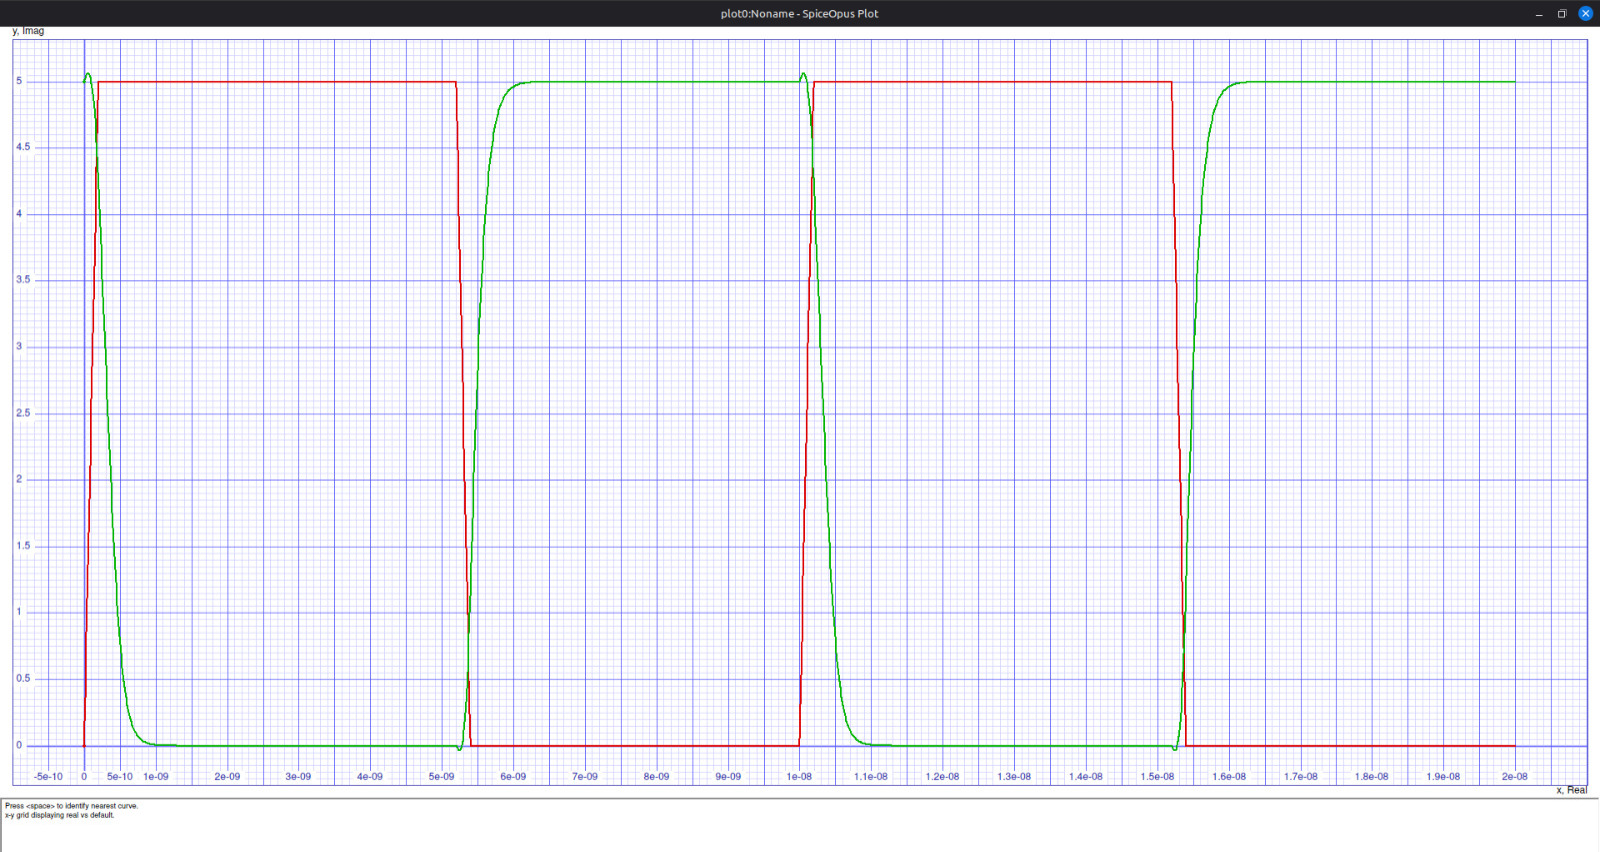
\includegraphics[width=\columnwidth]{1.jpeg}}
\caption{Gráfico da tensão de entrada e saída (plot tran1 v(in) v(out)).}
\label{fig1}
\end{figure}

Ao executar o comando para plotar a corrente, observou-se picos exatos nos instantes das transições lógicas, caracterizando o consumo dinâmico necessário para carregar o capacitor e a corrente de curto-circuito momentânea entre PMOS e NMOS (Fig. 2).

\begin{figure}[htbp]
\centerline{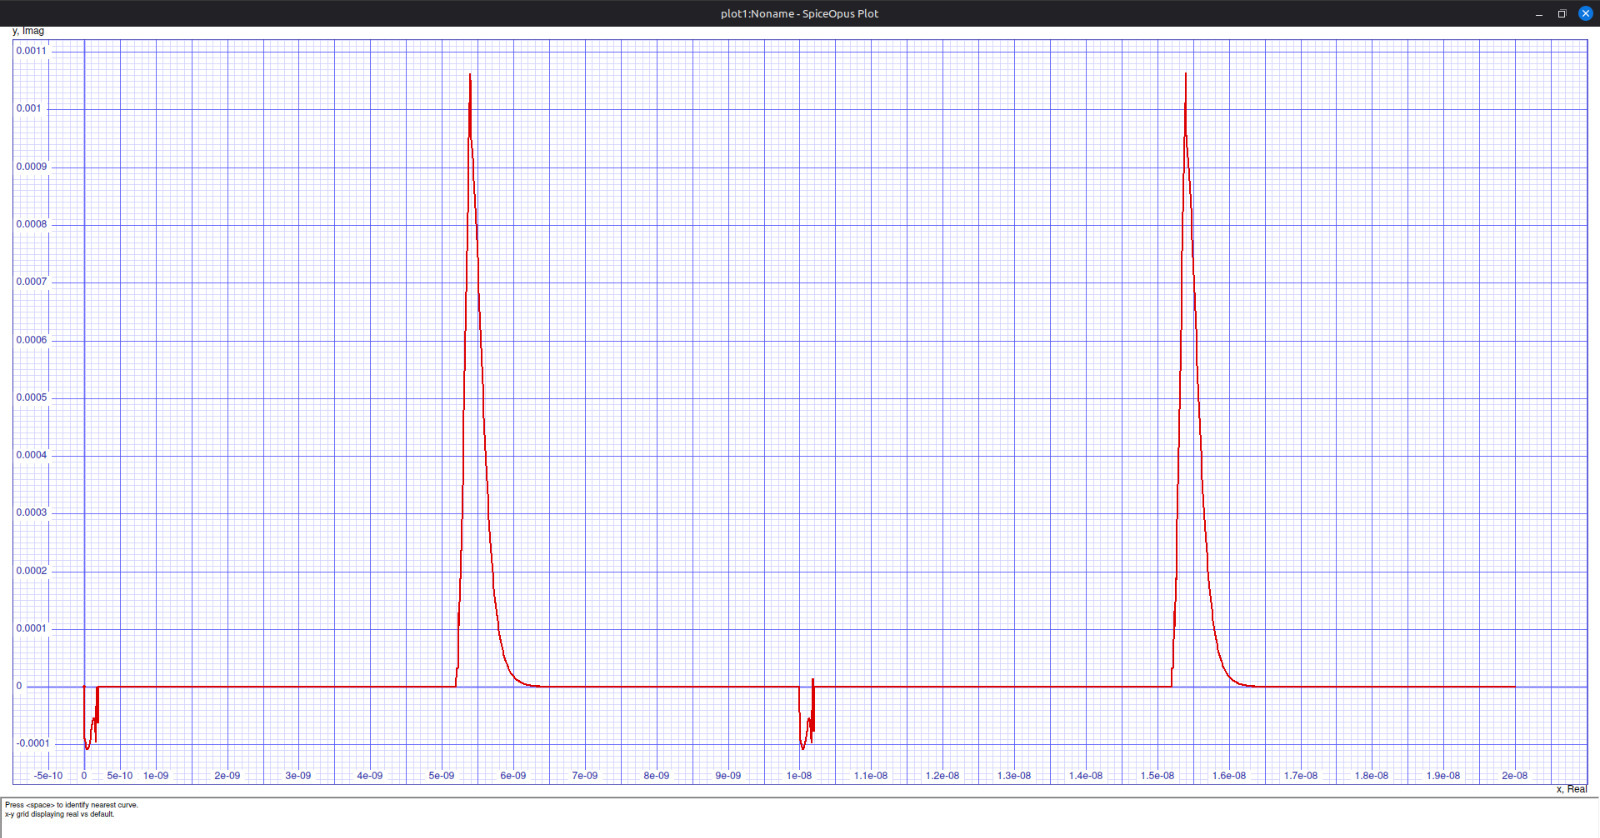
\includegraphics[width=\columnwidth]{2.jpeg}}
\caption{Corrente drenada da alimentação (plot i(Vdummy)) para 50fF.}
\label{fig2}
\end{figure}

\subsection{Atividade 02 - Inversor CMOS - Variações nos Parâmetros}
O objetivo desta etapa foi alterar características do circuito e avaliar os impactos físicos e temporais:

\subsubsection{Alteração da capacitância para 300fF}
Ao aumentar a capacitância para 300fF, a constante RC de saída do circuito aumentou significativamente. A duração e a área dos picos no gráfico de corrente também aumentaram (Fig. 3), pois é necessária mais energia para carregar uma carga capacitiva maior, tornando o circuito mais lento.

\begin{figure}[htbp]
\centerline{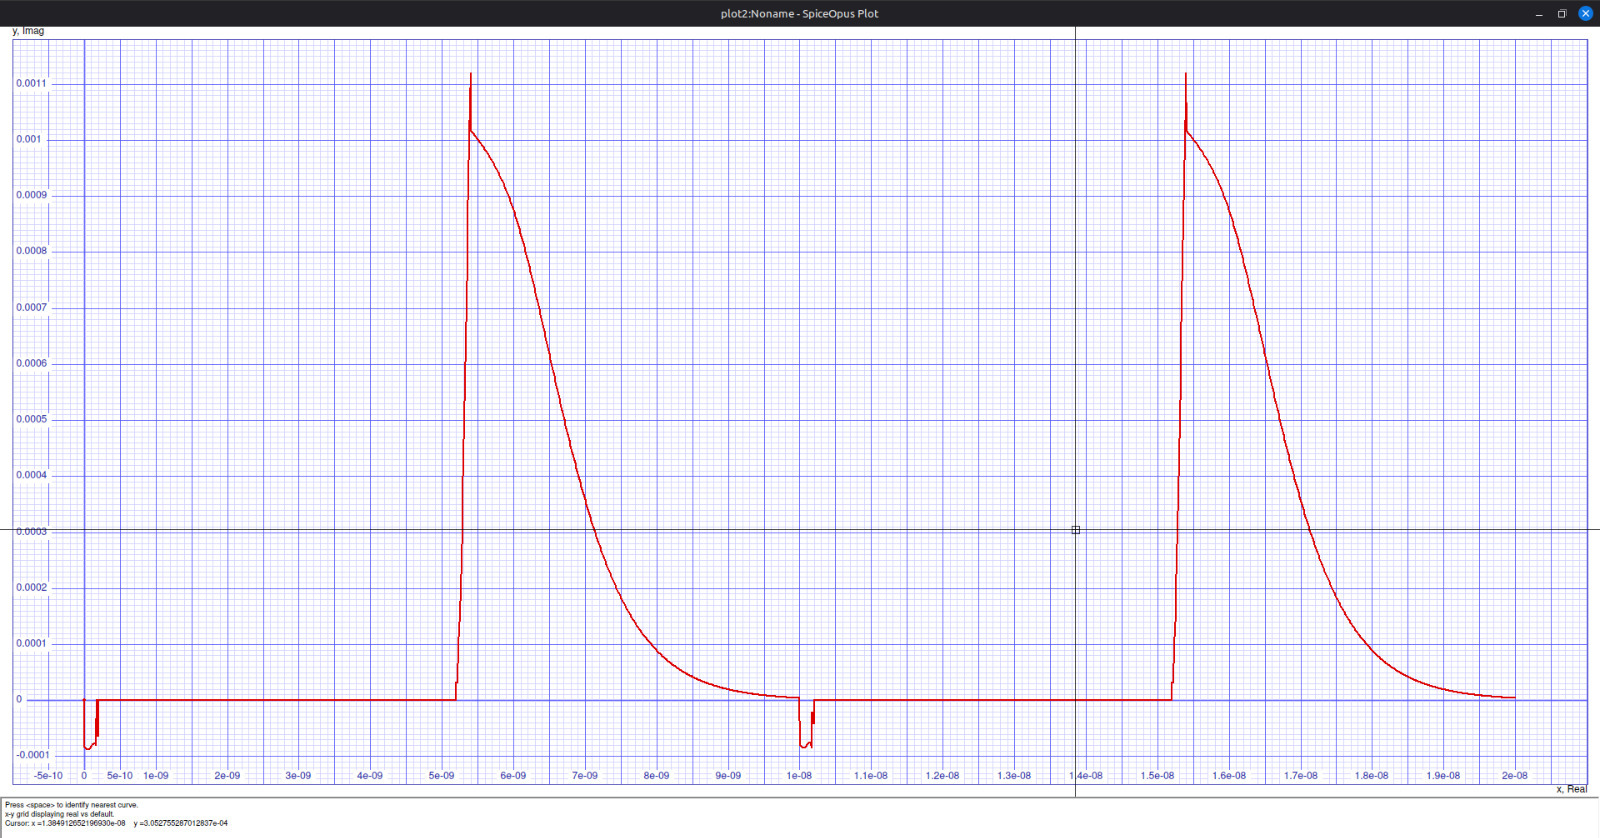
\includegraphics[width=\columnwidth]{3.jpeg}}
\caption{Pico de corrente com capacitância alterada para 300fF.}
\label{fig3}
\end{figure}

\subsubsection{Dobrando a largura (W) dos transistores}
Mantendo a capacitância em 300fF, o valor de $W$ foi dobrado. Um canal mais largo reduz a resistência de condução dos transistores. Isso gerou uma capacidade de fornecimento de corrente muito maior (Fig. 4), o que recarregou o capacitor mais rapidamente, diminuindo os atrasos temporais observados na etapa anterior.

\begin{figure}[htbp]
\centerline{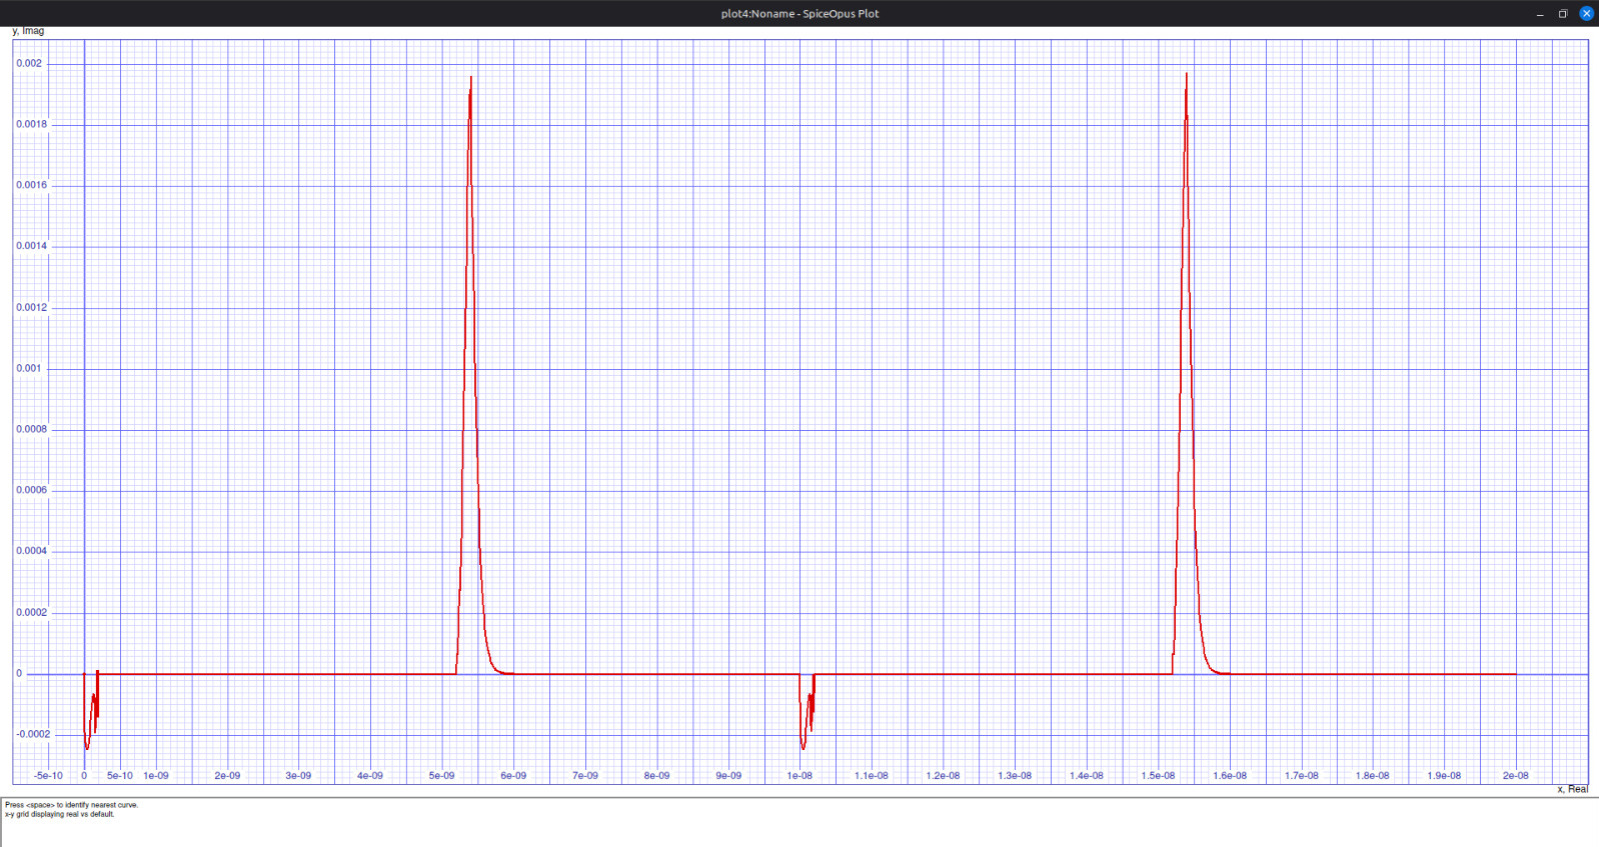
\includegraphics[width=\columnwidth]{4.jpeg}}
\caption{Corrente com capacitância em 300fF e largura W dobrada.}
\label{fig4}
\end{figure}

\subsubsection{Dobrando o comprimento (L) dos transistores}
Com $C_{out} = 300$fF e $W$ dobrado, o comprimento $L$ do canal também foi dobrado. O aumento de $L$ causa um aumento proporcional na resistência do canal, restringindo o fluxo de elétrons. Isso anulou o ganho de velocidade obtido no item anterior, degradando novamente os tempos de propagação e transição (Fig. 5).

\begin{figure}[htbp]
\centerline{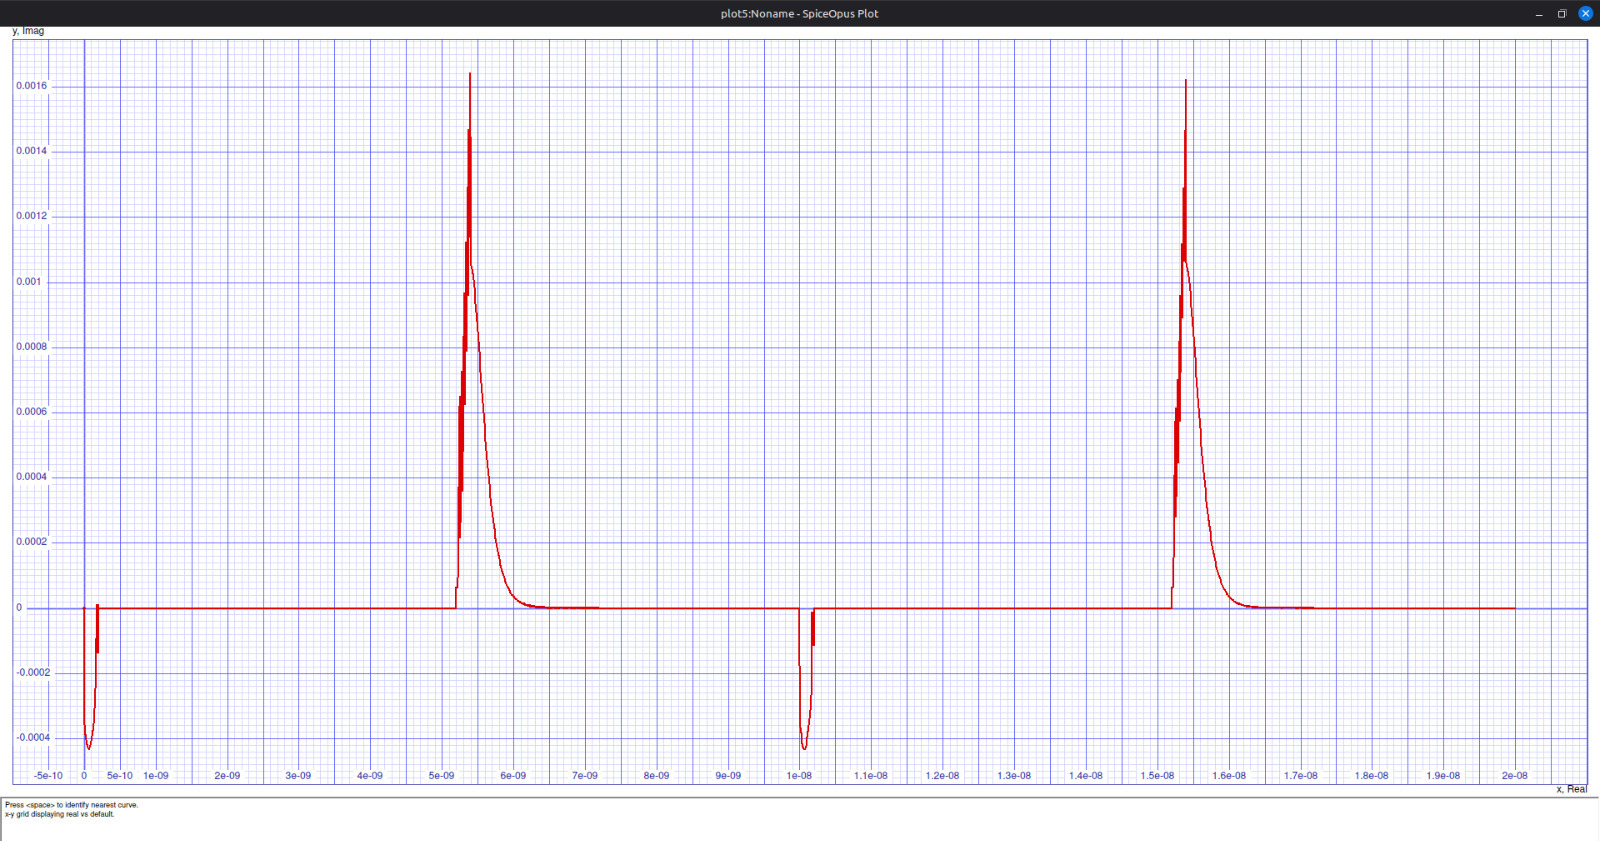
\includegraphics[width=\columnwidth]{5.jpeg}}
\caption{Comportamento do circuito após dobrar o comprimento L do canal.}
\label{fig5}
\end{figure}

\subsubsection{Potência Dissipada e Discussão Geral}
A potência dissipada dinamicamente pode ser obtida calculando a integral (a área sob a curva) do gráfico da corrente chaveada multiplicada pela tensão de alimentação de 5V ($P = V \cdot I$). As diferenças observadas ilustram o dilema de hardware: aumentar $W$ melhora o atraso ($T_{p}$) de cargas pesadas, mas aumenta o pico de corrente; aumentar a carga capacitiva compromete severamente a velocidade.

\section{Conclusões}
O Laboratório 04 foi imprescindível para unir a abstração lógica aos fundamentos eletrônicos de baixo nível. A ferramenta SpiceOpus provou-se altamente eficaz para visualizar os fenômenos transitórios que não podem ser vistos a olho nu ou modelados por tabelas-verdade.

Através das variações nos parâmetros, ficou evidente a influência geométrica dos transistores CMOS. Alterações físicas na largura ($W$) e no comprimento ($L$) do canal determinam a resistência do dispositivo, afetando a velocidade com que a carga é manipulada. Ficou claro que o desempenho otimizado exige mais energia de chaveamento, reafirmando que o design digital moderno baseia-se em trade-offs entre tamanho, atraso e consumo.

\begin{thebibliography}{00}
\bibitem{b1} R. A. L. Reis, \textit{Concepção de Circuitos Integrados}. Porto Alegre: Bookman, 2009.
\bibitem{b2} J. P. Uyemura, \textit{Sistemas digitais: uma abordagem integrada}. São Paulo: Thomson/Pioneira, 2002.
\bibitem{b3} R. Tocci, N. Widmer, and G. Moss, \textit{Sistemas Digitais - Princípios e Aplicações}, 12th ed. São Paulo: Pearson, 2018.
\end{thebibliography}

\end{document}
